\documentclass{article}
    \usepackage{float}
    \usepackage{textcomp}
    \usepackage{graphicx}
    \usepackage{booktabs}
    \usepackage{color}
    \usepackage{verbatim}
    \usepackage{listings}
    \usepackage{underscore}
    \usepackage{amsmath}
    \usepackage{amssymb}
    %\usepackage{showkeys}
    %\usepackage{float} % here for H placement parameter
    \usepackage{flafter} 
    \setcounter{secnumdepth}{5}
    \usepackage[bookmarks=true]{hyperref}
    \author{\textbf{Marco Bissessur}} 
    \date{20 Giugno 2018}
    \title{ITIS G. Feltrinelli
        \\A.A. 2017\@-\@2018
        \\Documentazione tesina maturità \\ \textbf{Badminton Clubs}
      } 
        \hypersetup{pdftitle={Documentazione},    % title
        pdfauthor={Marco Bissessur},                     % author
        pdfsubject={tesina},                        % subject of the document
        colorlinks=true,       % false: boxed links; true: colored links
        linkcolor=blue,       % color of internal links
        citecolor=blue,       % color of links to bibliography
        filecolor=black,        % color of file links
        urlcolor=blue,        % color of external links
       }
    \begin{document}
    \maketitle
    \begin{center}
        \includegraphics[width=7cm]{logofeltrinelli}
    \end{center}
    \clearpage
    {\hypersetup{hidelinks}\tableofcontents}
    \clearpage
    
    \section{Introduzione}

    \section{Obiettivo}
%L'Obiettivo principale di Badminton Clubs è di aiutare gli utenti a organizzare tornei tra amici o con altri utenti, formare gruppi di amici o incontrare nuove persone attraverso club e  
L'Obiettivo principale di Badminton Clubs è di creare un social network che permetta   agli utenti di organizzare e gestire tornei tra di loro, nello specifico voglio creare un prodotto che possa:
\begin{itemize}
    \item Permettere agli utenti di inviare richieste di amicizia, accettarle e visuallizare gli amici
    \item Permettere agli utenti di creare tornei con nome, descrizione, numero di partecipanti, tipo di torneo (singolo, doppio) e il sesso dei partecipanti. Gestirli e organizzare i turni.
    \item Permettere agli utenti di creare club e fare gruppi tra di loro.
    \item Permettere agli utenti  di visuallizare i club in base ad una classifica in base al loro punteggio.
    \item Permettere di visualizzare gli utenti iscritti e gli ultimi tornei creati
\end{itemize}
\section{Requisiti funzionali}

    \section{Tecnologia utilizzata}
    \subsection{Front end}
    \subsubsection{Linguaggi}
 I linguaggi Front end che ho utilizzato sono:
 \begin{itemize}
    \item HTML per creare la struttura base delle pagine dell'applicazione
    \item CSS per modellare la pagina e renderla responsive 
    \item JAVASCRIPT per creare animazioni, e soprattutto per la creazione dinamica
    dell'albero che rappresenta i vari match di un torneo.
  \end{itemize}
    \subsection{Back end}
    \subsubsection{Linguaggi}
Per programmare il back end ho utilizzato il linguaggio PHP, per creare contenuto
dinamico nelle pagine, i cui dati sono presi tramite query
dal database MySql.
\subsubsection{Hosting}
L'applicazione è stata pubblicata sul dominio https://www.marcobissessur.it affittato
da Aruba srl, la gestione del database è avvenuta come per il 
database locale di MAMP.



\subsection{Database}
    Questo è lo schema UML della struttura del database progettato con MySql
    \begin{center}
        \includegraphics[width=15cm]{images/schemapng}
    \end{center}
    \subsubsection{Users}
    \begin{center}
        \includegraphics[width=15cm]{images/users}
    \end{center}
    \subsubsection{Club}
    \begin{center}
        \includegraphics[width=15cm]{images/club}
    \end{center} 
    \subsubsection{Club Ranking}
    \begin{center}
        \includegraphics[width=15cm]{images/rankingclub}
    \end{center}
    \subsubsection{User images}
    \begin{center}
        \includegraphics[width=15cm]{images/userimages}
    \end{center}
    \subsubsection{Tournament}
    \begin{center}
        \includegraphics[width=15cm]{images/tournament}
    \end{center}
    \subsubsection{Participant}
    \begin{center}
        \includegraphics[width=15cm]{images/participant}
    \end{center}
    \subsubsection{Friendship}
    \begin{center}
        \includegraphics[width=15cm]{images/friendship}
    \end{center}
    \subsubsection{Friend Request}
    \begin{center}
        \includegraphics[width=15cm]{images/friendrequest}
    \end{center}
    \subsubsection{Club member}
    \begin{center}
        \includegraphics[width=15cm]{images/clubmember}
    \end{center}

    \section{Use cases}
    tabelle con omini
    spiegazione delle tabelle, es. come l'admin del torneo gestisce il torneo

    \begin{center}
        Un utente può cercare il torneo in cui vuole partecipare, può unirsi dopo aver visto le caratteristiche del torneo e aspetta che esso si svolga. \\ 
        Poi l'admin del torneo ovvero il suo creatore assegna i vincitori dei match man mano che si svolgono fino a quando non c'è un vincitore finale.\\
        Ogni volta che un utente vince un match, li viene assegnato un punteggio in base all'importanza del match.
        \includegraphics[width=18cm]{UX/tournament-usecase}
    \end{center}
Un utente quando visita la pagina di altri utenti può mandare a loro una richiesta di amicizia, e il destinatario può decidere se accettare o declinare la richiesta.
    \begin{center}
        \includegraphics[width=18cm]{UX/profile-usecase}
    \end{center}
L'admin dopo aver creato il club può decidere se uscire o no, gli utenti invece scelgono se entrare nel club o uscirne. Se un utente è gia dentro un club, quando cerca altri club può scegliere se uscire dal proprio club.
    \begin{center}
        \includegraphics[width=18cm]{UX/club-usecase}
    \end{center}

    \section{UX user experience}
    \subsection{ Navigazione delle pagine }
   
    \begin{center}
        \includegraphics[width=18cm]{UX/BadmintonUX}
    \end{center}
    \subsection{Sign up}
Un nuovo utente dalla pagina di Login va nella pagina di Sign up, si registra e se non compila tutti i campi torna nella stessa pagina, altrimenti viene\\ reindirizzato alla pagina di Login. \\
\begin{center}
    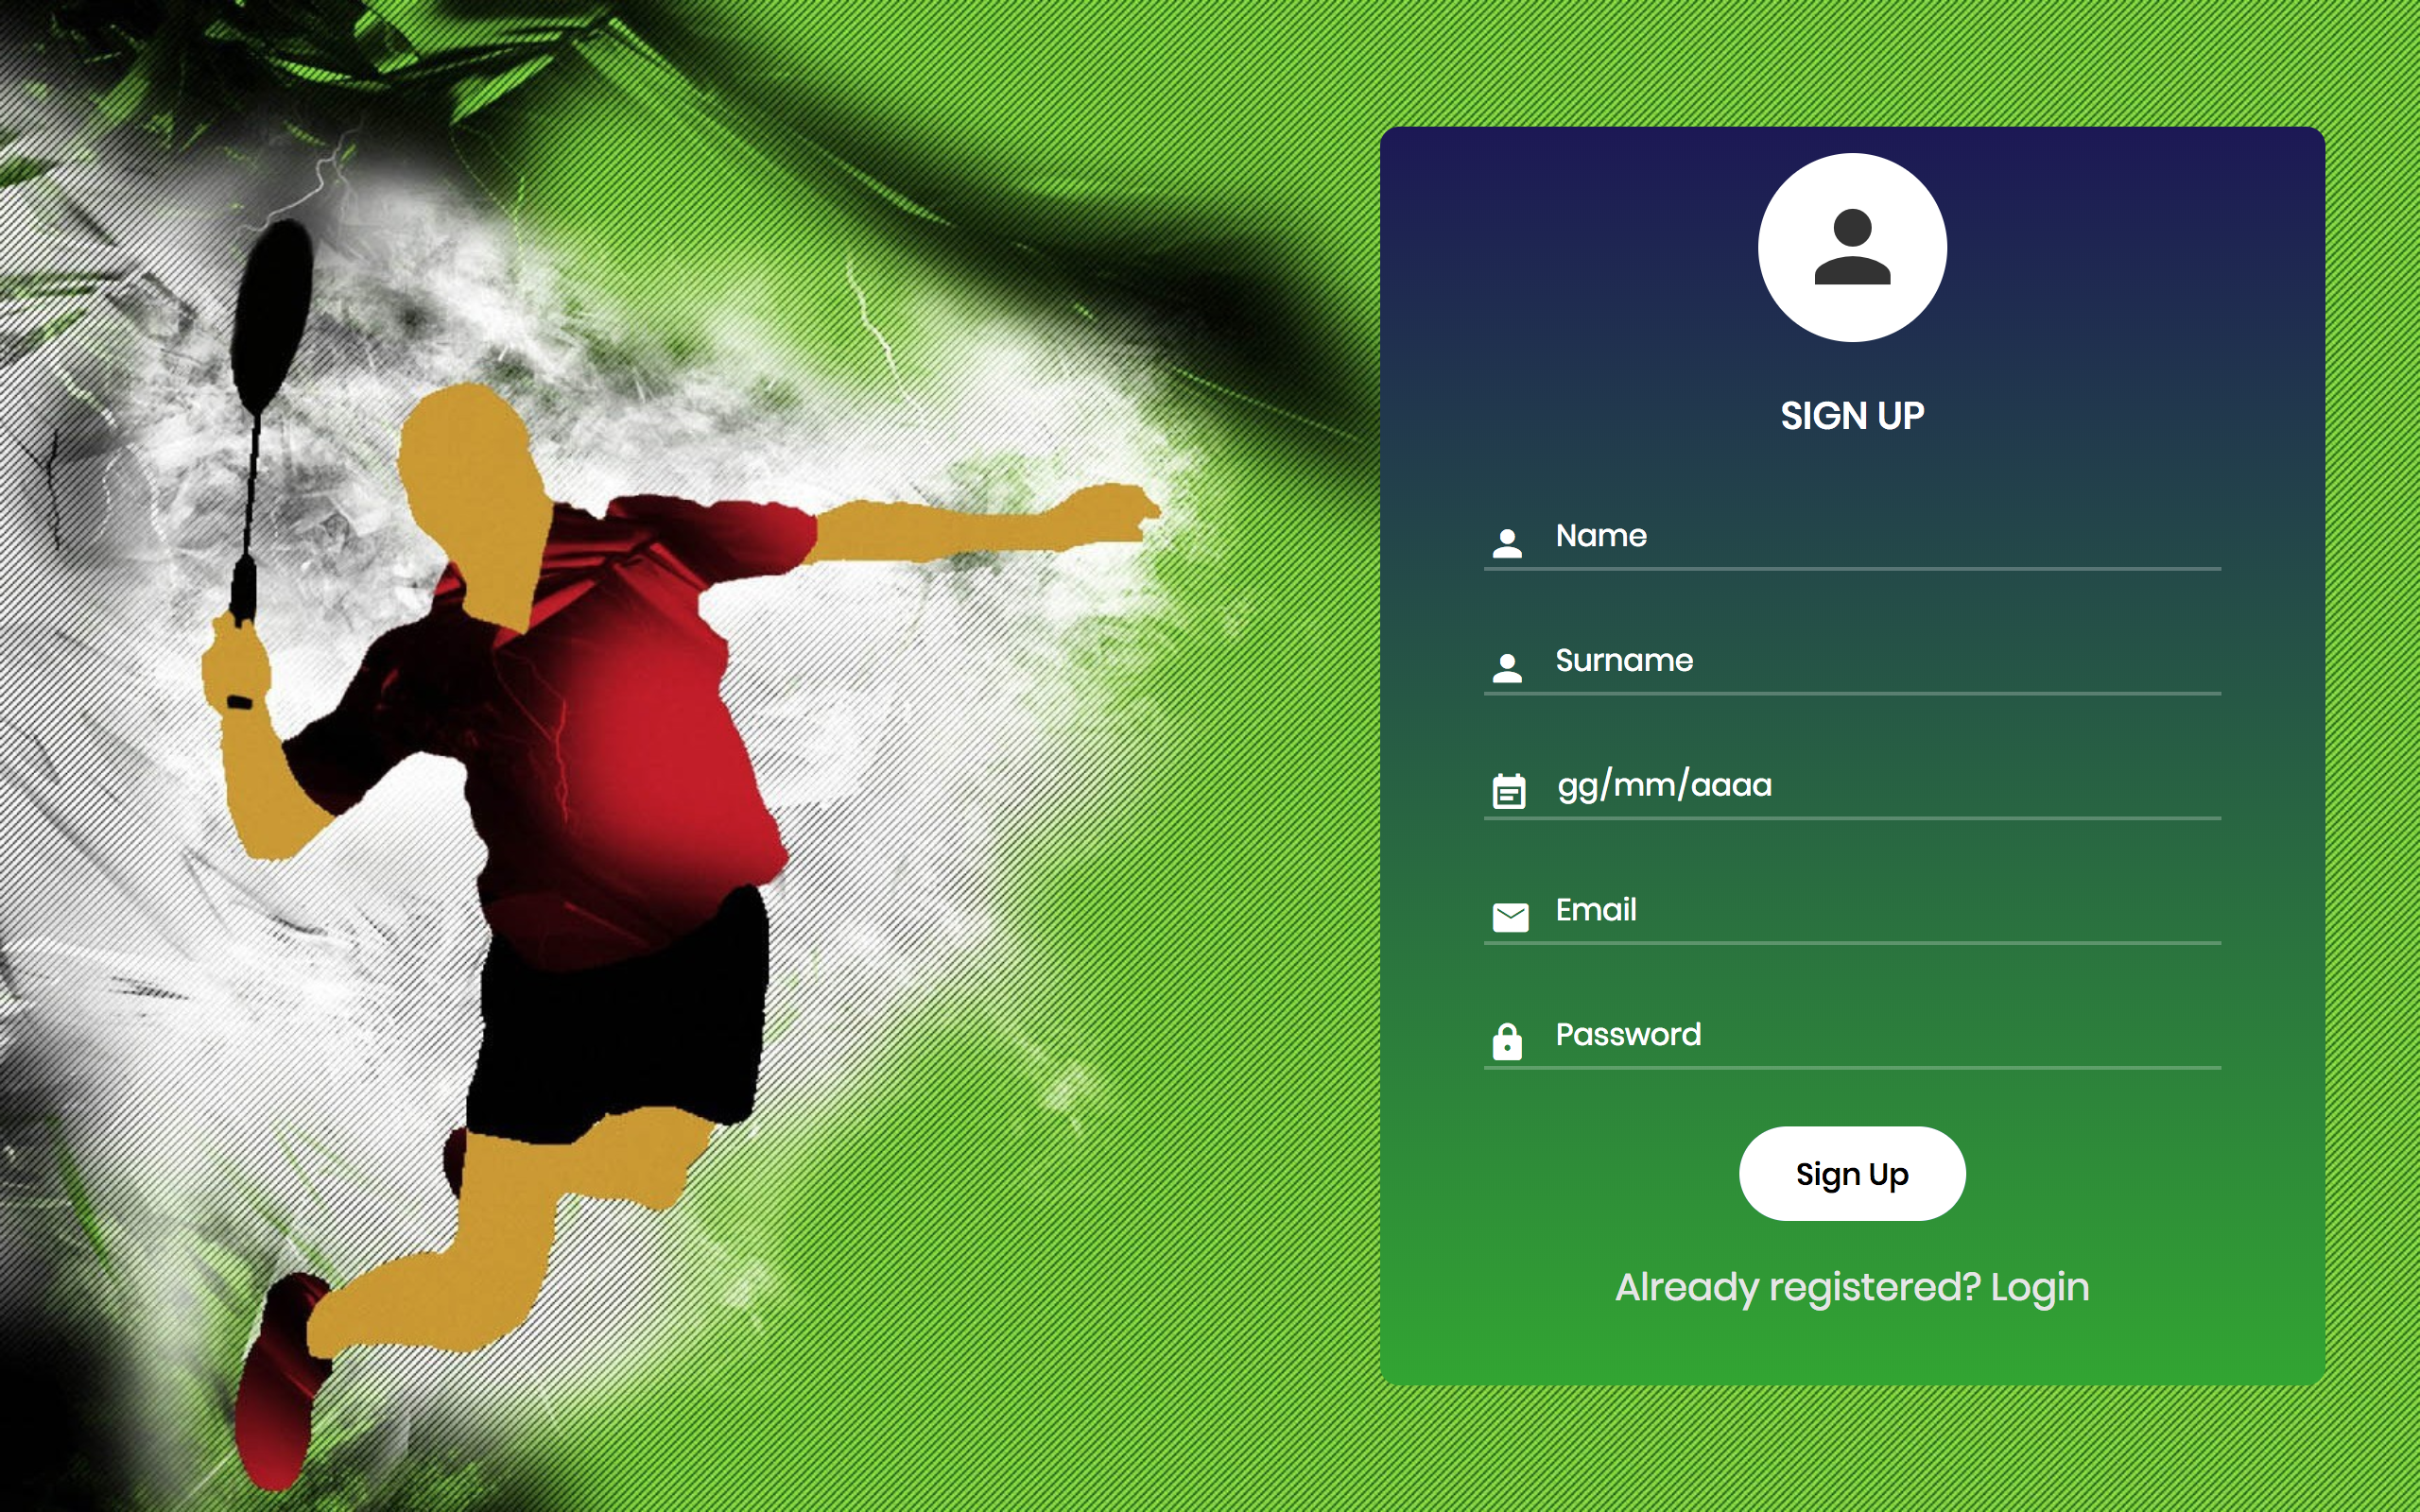
\includegraphics[width=16cm]{UX/signup}
\end{center}
\subsection{Login}
Nel Login se inserisce credenziale errate rimane nella pagina, se invece inserisce delle credenziale valide viene reindirizzato alla Homepage del sito.\\
\begin{center}
    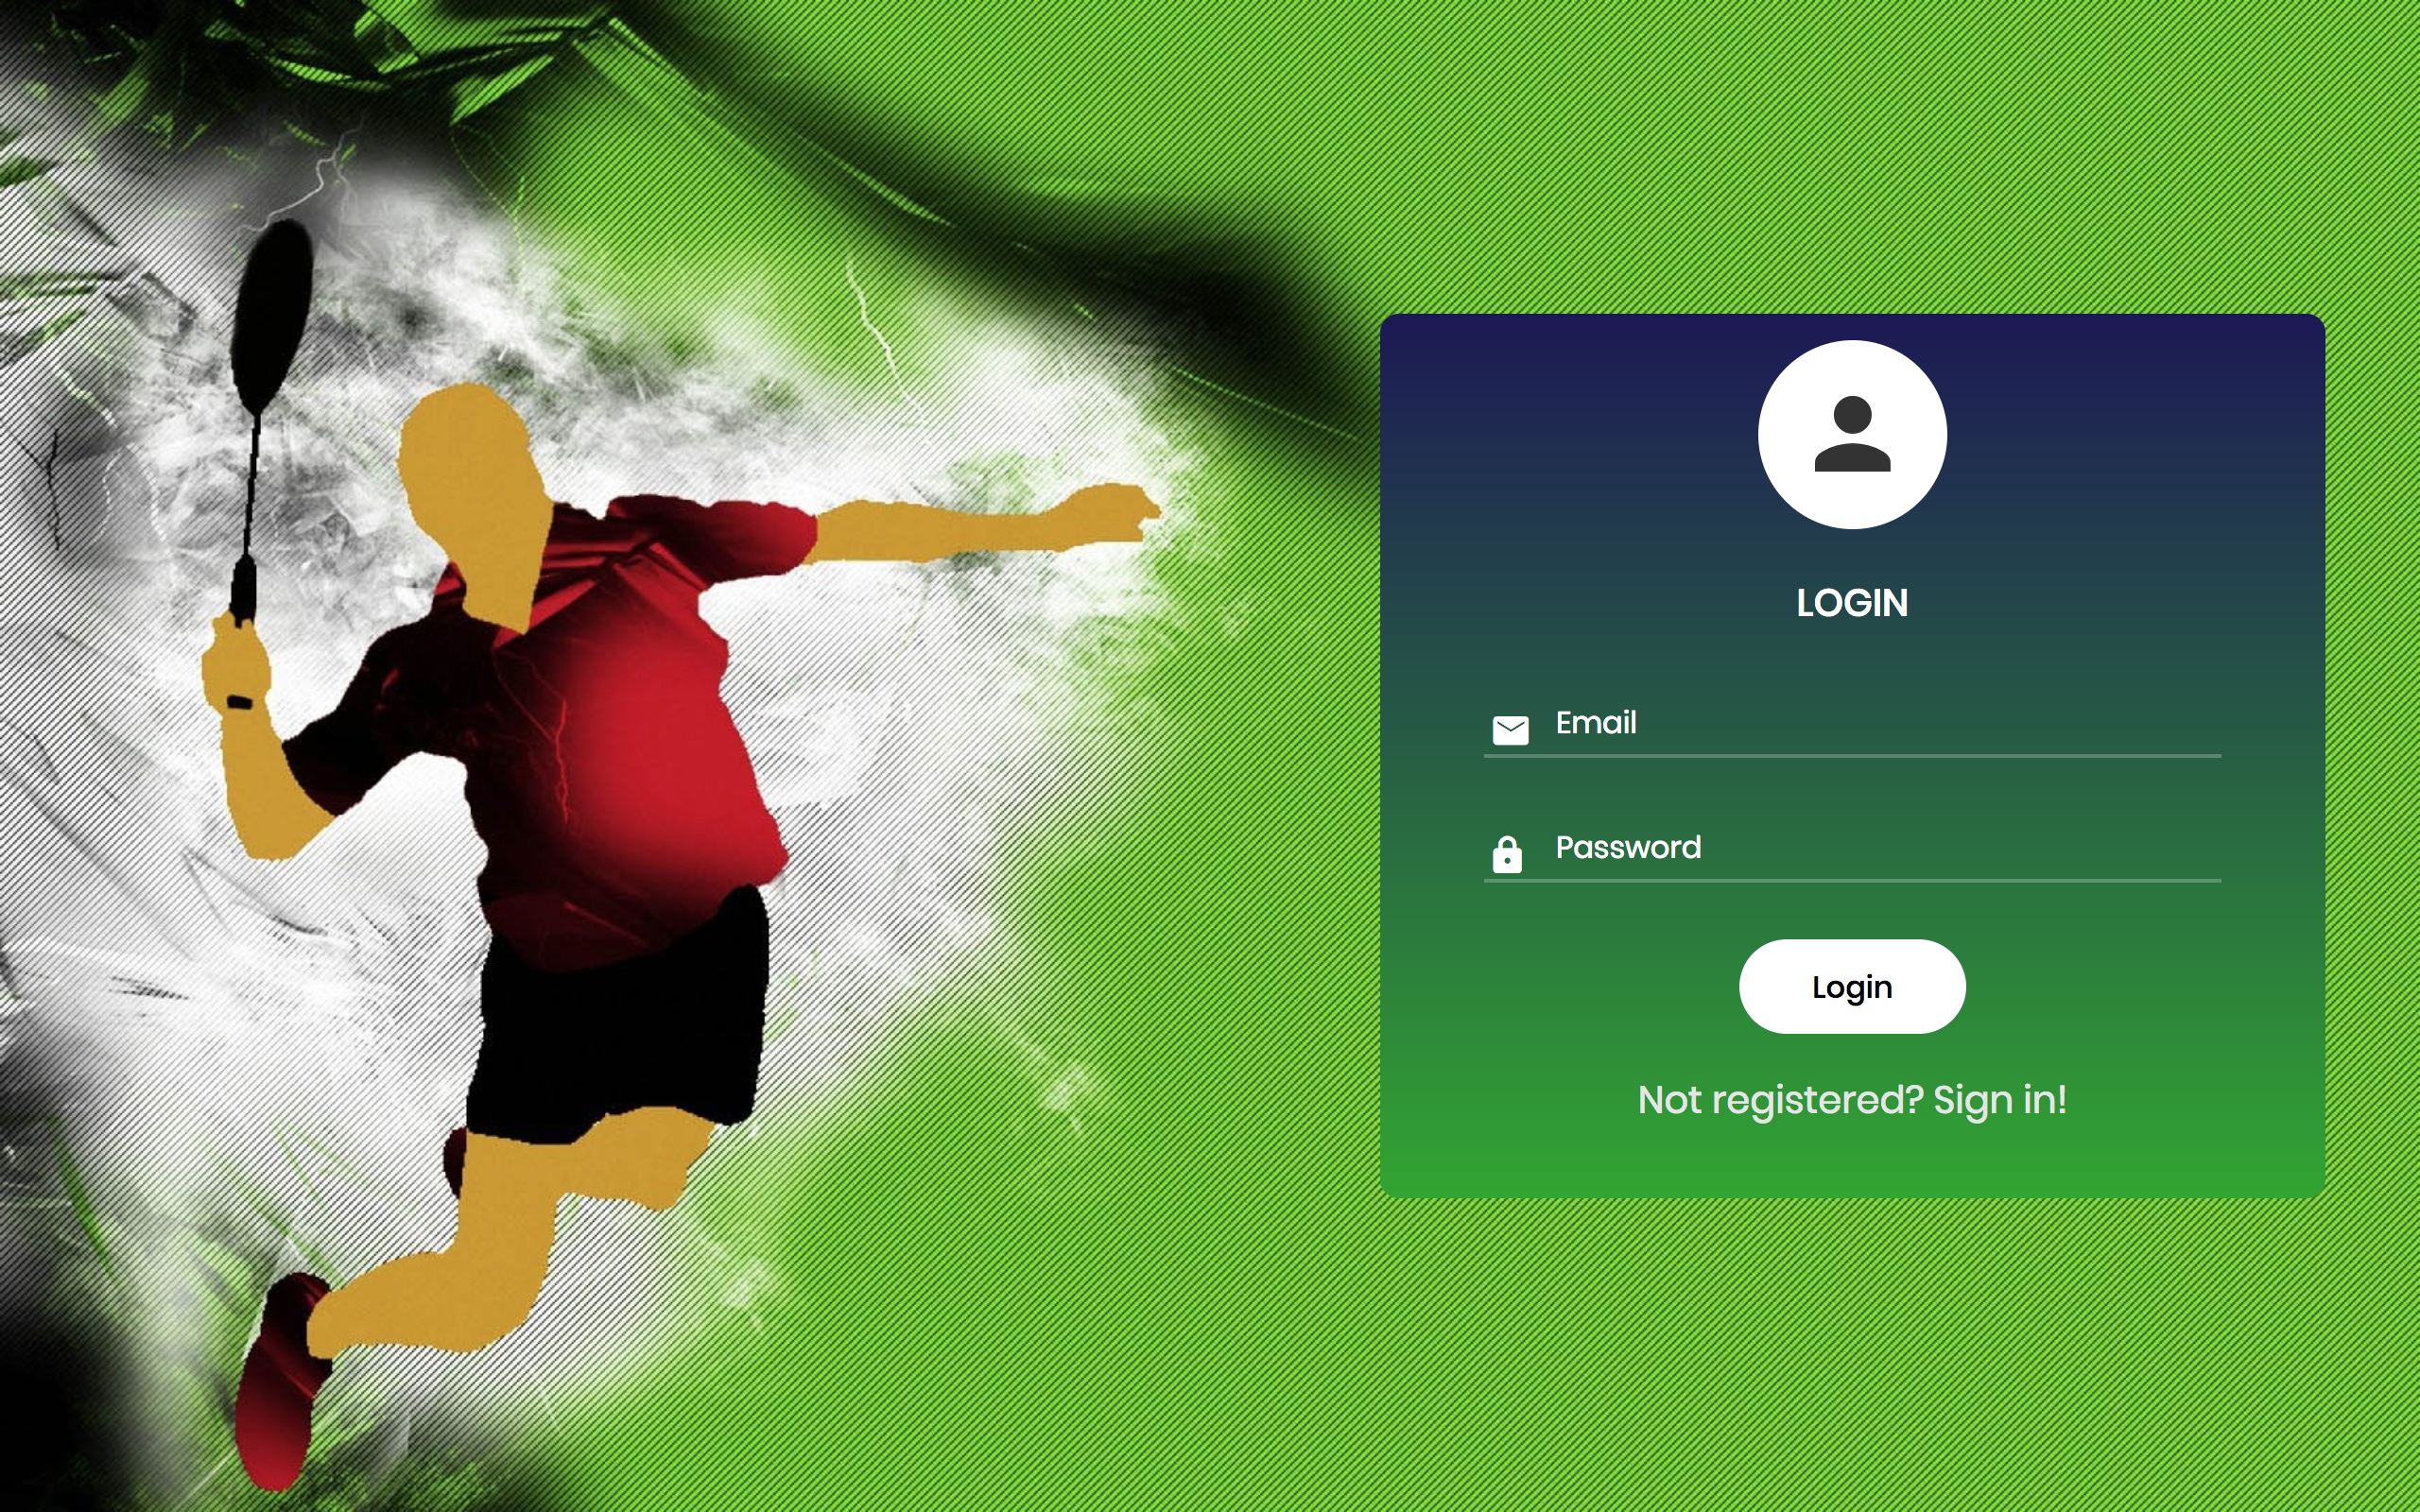
\includegraphics[width=16cm]{UX/login}
\end{center}
\subsection{Homepage}
Nella Homepage l'utente può visualizzare: 
\begin{itemize}
    \item Gli ultimi 4 utenti registrati 
    \item I migliori 7 club con i loro punteggi
    \item Gli ultimi 4 tornei creati
    \item I 3 utenti migliori dell'applicazione
  \end{itemize}
    
  \begin{center}
    \includegraphics[width=16cm]{UX/hometop}
\end{center}
\begin{center}
    \includegraphics[width=16cm]{UX/homebot}
\end{center}
\subsection{Navbar}
Nella barra di navigazione l'utente può andare all'homepage cliccando su Badminton Clubs, nelle impostazioni cliccando Settings e nel suo profilo cliccando su MyProfile.
\begin{center}
    \includegraphics[width=16cm]{UX/navbar}
\end{center}
Se l'utente non appartiene a nessun club può crearne uno.\\
L'utente può anche cercare: un altro utente, un club o un torneo inserendo il nome di uno di essi nel campo di ricerca.\\
Cliccando il campo Request si può controllare se qualcuno ha inviato delle richieste di amicizia e decidere se accettarle o meno.\\
Infine l'utente può anche decidere di effetuare il logout.

\subsection{MyProfile}
Nella pagina MyProfile l'utente cliccando sull'immagine sopra il suo nome (es. Nuovo Utente) può caricare la sua immagine di profilo principale,\\ che si vedrà anche nella barra di navigazione.
\\A destra invece l'utente può caricare altre 4 immagini visibili solo nel suo profilo. 
\begin{center}
    \includegraphics[width=16cm]{UX/mypnuovo}
\end{center}
Dopo aver caricare le foto il profilo verrà simile al seguente esempio:
\begin{center}
    \includegraphics[width=16cm]{UX/myp}
\end{center}
Nella pagina si può anche controllare le tue skills:
\begin{itemize}
    \item [Win Rate] Percentuale di vittorie di tornei partecipati
    \item [Club Points] Punti del tuo club e posizione complessiva 
    \item [Global Rank] Posizione personale nel ranking globale
  \end{itemize}
\begin{center}
    \includegraphics[width=16cm]{UX/mypskills}
\end{center}
Si possono anche visualizzare i tornei svolti o in corso e visitarli
\begin{center}
    \includegraphics[width=16cm]{UX/myptour}
\end{center}
E visualizzare i tuoi amici e i loro profili
\begin{center}
    \includegraphics[width=16cm]{UX/mypfriendsl}
\end{center}




\section{Workflow}

Per fare il social network ho utilizzato MAMP per lavorare in locale sul mio computer, L'IDE che ho utilizzato è Brackets che ho usato per programmare le pagine front e back end. Ho utilizzanto git come Version Control System per gestire il workflow, infine ho pubblicato l'applicazione su un dominio online 
(\href{https://www.marcobissessur.it}{Badminton Clubs}). \\
Per la Documentazione ho utlizzato il linguaggio Latex e Visual Studio Code come IDE.
    

    
    
    \end{document}